\documentclass[UTF8,a4paper,12pt,fontset=none]{ctexart}

\usepackage[a4paper,margin=2.2cm]{geometry}
\usepackage{amsmath}
\usepackage{amssymb}
\usepackage{array}
\usepackage{booktabs}
\usepackage{caption}
\usepackage{enumitem}
\usepackage{float}
\usepackage{fontspec}
\usepackage{graphicx}
\usepackage{hyperref}
\usepackage{listings}
\usepackage{siunitx}
\usepackage{subcaption}
\usepackage{tabularx}
\usepackage{xurl}
\usepackage{xcolor}

\hypersetup{colorlinks=true,linkcolor=blue!60!black,urlcolor=blue!60!black}
\defaultCJKfontfeatures{AutoFakeSlant=.2}
\setCJKmainfont{Songti SC}
\setCJKsansfont{Heiti SC}
\setCJKmonofont{Heiti SC}
\setmonofont{Menlo}
\setlength{\parindent}{2em}
\setlength{\parskip}{0.35em}
\emergencystretch=3em
\graphicspath{{../results/figures/}}
\captionsetup{font=small}
\sisetup{round-mode=places,round-precision=3}
\renewcommand{\figurename}{图}
\renewcommand{\tablename}{表}

\definecolor{CodeBg}{HTML}{F7F7F7}
\definecolor{CodeKeyword}{HTML}{1D4E89}
\definecolor{CodeComment}{HTML}{0B6E4F}
\definecolor{CodeString}{HTML}{C73E1D}

\lstset{
  basicstyle=\ttfamily\small,
  backgroundcolor=\color{CodeBg},
  frame=single,
  framerule=0pt,
  xleftmargin=1em,
  xrightmargin=1em,
  breaklines=true,
  columns=fullflexible,
  keywordstyle=\color{CodeKeyword}\bfseries,
  commentstyle=\color{CodeComment},
  stringstyle=\color{CodeString},
  showstringspaces=false
}

\title{\bfseries 中山大学计算机学院本科生实验报告}
\author{}
\date{}

\begin{document}

\begin{titlepage}
  \centering
  {\zihao{2}\bfseries 中山大学计算机学院本科生实验报告\par}
  \vspace{0.5em}
  {\zihao{4}（2025学年春季学期）\par}
  \vspace{2em}

  \begin{tabularx}{0.9\textwidth}{>{\bfseries}p{4cm}X}
    课程名称： & 并行程序设计与算法 \\
    实验题目： & Lab11 CUDA卷积计算 —— 多策略并行卷积与cuDNN对比 \\
    批改人： & \\
    专业（方向）： & \\
    学号： & 23336128 \\
    姓名： & 梁力航 \\
    Email： & \\
    完成日期： & 2026年6月12日 \\
  \end{tabularx}

  \vfill
  \begin{minipage}{0.88\textwidth}
    \small
    本次实验使用CUDA实现了4种CNN卷积计算方法（朴素直接卷积、共享内存分块卷积、
    im2col+GEMM变换、cuDNN库卷积），在智算习堂RTX 3090平台上测试了8种输入规模
    （32--4096）和3种stride（1/2/3）。实验发现：在3×3小卷积核场景下，tiled\_conv
    仅比naive\_conv快约2--3\%，而cuDNN受限于sm\_37编译器目标反而比手写kernel
    慢约28\%，揭示了编译器与GPU代际匹配对库函数性能的重要性。
  \end{minipage}
\end{titlepage}

\section{实验目的}

\begin{enumerate}[leftmargin=2.2em]
  \item 掌握CUDA卷积计算的多种并行策略：直接滑窗（全局内存）、共享内存分块（含halo区域）、
        算法变换（im2col+GEMM）以及库函数调用（cuDNN）；
  \item 理解不同并行方法对3×3卷积这一访存密集型操作的适用性，分析共享内存tiling在小卷积核下
        的收益与代价；
  \item 学习cuDNN卷积接口的使用，对比库函数与手写kernel的实际性能差异；
  \item 分析stride、输入规模、block大小等参数对各卷积kernel性能的影响规律。
\end{enumerate}

\section{实验平台与工具链}

\begin{table}[H]
  \centering
  \caption{实验平台与工具链}
  \label{tab:platform}
  \begin{tabular}{ll}
    \toprule
    项目 & 参数 \\
    \midrule
    GPU & NVIDIA GeForce RTX 3090 (GA102, Ampere SM 8.6) \\
    CUDA核心 & 10,496 \\
    显存 & 24 GB GDDR6X，带宽 936 GB/s \\
    共享内存/Block & 最大 48 KB（可配置至 100 KB） \\
    Warp大小 & 32，最大线程/Block = 1024 \\
    \midrule
    CUDA Toolkit & nvcc 10.0 (2018)，编译目标 sm\_37 \\
    CUDA Runtime & 12.x（pip nvidia-cuda-runtime-cu12 提供） \\
    cuDNN & 8.9.7（pip nvidia-cudnn-cu12 提供，替换系统7.6.5） \\
    C++标准 & C++14, -O3 \\
    \midrule
    计算平台 & 智算习堂（中山大学GPU计算平台） \\
    本地环境 & Apple M4, macOS Sequoia \\
    Python & 平台 3.8（benchmark/plot脚本） \\
    \bottomrule
  \end{tabular}
\end{table}

\textbf{关于CUDA/cuDNN版本的说明}：平台系统的CUDA Toolkit 10.0（2018年版本）
配套cuDNN 7.6.5，无法在RTX 3090（Ampere架构）上初始化。实验通过pip安装新版
cuDNN 8.9.7和CUDA Runtime 12.x，编译仍使用nvcc 10.0（sm\_37目标），运行时通过
LD\_LIBRARY\_PATH加载新版动态库。这一方案使cuDNN能正常运行，但编译器降级
（sm\_37 PTX经JIT到sm\_86）影响了cuDNN内核的优化效果。

\section{问题描述与算法设计}

\subsection{CNN卷积问题定义}

给定输入张量 $I \in \mathbb{R}^{C_{in} \times H \times W}$ 和卷积核
$K \in \mathbb{R}^{C_{out} \times C_{in} \times KH \times KW}$，2D卷积输出
$O \in \mathbb{R}^{C_{out} \times H_{out} \times W_{out}}$ 为：

\begin{equation}
  O[c_o][y][x] = \sum_{c_i=0}^{C_{in}-1} \sum_{k_y=0}^{KH-1} \sum_{k_x=0}^{KW-1}
  I[c_i][y \cdot S + k_y - P][x \cdot S + k_x - P] \cdot K[c_o][c_i][k_y][k_x]
\end{equation}

其中 $S$ 为stride，$P$ 为padding。本次实验固定 $C_{in}=C_{out}=3$, $KH=KW=3$,
$P=1$，不包含卷积核翻转（实现为cross-correlation）和bias。输出尺寸为：

\begin{equation}
  H_{out} = \lfloor \frac{H + 2P - KH}{S} \rfloor + 1,
  \quad W_{out} = \lfloor \frac{W + 2P - KW}{S} \rfloor + 1
\end{equation}

\subsection{四种卷积Kernel概览}

\begin{table}[H]
  \centering
  \caption{四种卷积Kernel的方法特征}
  \label{tab:kernels}
  \begin{tabular}{lccc}
    \toprule
    Kernel & 方法 & 使用共享内存 & Block大小可配置 \\
    \midrule
    naive\_conv  & 直接滑窗，纯全局内存 & 否 & 是（8×8, 16×16, 32×32） \\
    tiled\_conv  & 直接滑窗，共享内存分块含halo & 是 & 否（固定16×16） \\
    im2col\_gemm & im2col展开 + 分块GEMM & 是（GEMM共用） & 否（自适应16/32） \\
    cudnn        & cuDNN cudnnConvolutionForward & 库内部管理 & -- \\
    \bottomrule
  \end{tabular}
\end{table}

\subsection{Kernel 1：朴素直接卷积（Naive）}

最直观的并行化：每个线程对应输出张量的一个元素 $(c_o, y, x)$，直接从全局内存
读取所有需要的输入和权值。Grid配置为3D：
$\lceil W_{out}/B_x \rceil \times \lceil H_{out}/B_y \rceil \times C_{out}$。

对于 $3\times3\times3=27$ 个权值和对应输入，每个输出元素需54次全局内存读取
（27次读input + 27次读weight），仅27次乘加（54 FLOPs），计算/访存比约
1 FLOP/load，是典型的访存密集型操作。

\begin{lstlisting}[language=C++, caption={朴素卷积Kernel}]
__global__ void convNaive(const float *input, const float *weight, float *output,
    int C, int H, int W, int KH, int KW,
    int H_out, int W_out, int stride, int padding) {

    int ox = blockIdx.x * blockDim.x + threadIdx.x;
    int oy = blockIdx.y * blockDim.y + threadIdx.y;
    int co = blockIdx.z;
    if (ox >= W_out || oy >= H_out) return;

    float sum = 0.0f;
    for (int ci = 0; ci < C; ++ci)
        for (int ky = 0; ky < KH; ++ky)
            for (int kx = 0; kx < KW; ++kx) {
                int iy = oy * stride + ky - padding;
                int ix = ox * stride + kx - padding;
                if (iy >= 0 && iy < H && ix >= 0 && ix < W)
                    sum += input[(ci*H+iy)*W+ix] * weight[((co*C+ci)*KH+ky)*KW+kx];
            }
    output[(co*H_out+oy)*W_out+ox] = sum;
}
\end{lstlisting}

\subsection{Kernel 2：共享内存分块卷积（Tiled）}

利用共享内存缓存输入数据的一个tile（含halo区域），让block内线程复用相邻的输入数据。
核心设计参数：

\begin{itemize}
  \item \textbf{Tile尺寸计算}：stride最大为3，halo区域需覆盖 $(B-1)\times3+KH$ 输入范围。
        对于 $B=16$：最大输入tile = $15\times3+3=48$，共享内存占用 $48\times48\times4\text{B}
        = 9\text{KB}$，在48KB限制内；
  \item \textbf{协作加载}：block内 $16\times16=256$ 个线程分工将输入tile的全部通道（C=3）
        依次载入共享内存。边缘线程处理越界填充（padding=1导致的部分输入位置无数据）；
  \item \textbf{权重存寄存器}：$3\times3\times3=27$ 个float直接放寄存器，不占用共享内存。
\end{itemize}

与Lab10的GEMM tiling不同，卷积tiling的收益来自输入数据的空间复用（相邻输出位置共享
大量输入元素），而非沿K维度的累加复用。

\begin{lstlisting}[language=C++, caption={共享内存分块卷积Kernel（协作加载+halo处理）}]
__global__ void convTiled(const float *input, const float *weight, float *output,
    int C, int H, int W, int KH, int KW,
    int H_out, int W_out, int stride, int padding) {

    __shared__ float tile[CONV_TILE_MAX_H][CONV_TILE_MAX_W]; // 48x48

    int ox = blockIdx.x * CONV_TILE_DIM + threadIdx.x;
    int oy = blockIdx.y * CONV_TILE_DIM + threadIdx.y;
    int co = blockIdx.z;
    float sum = 0.0f;

    for (int ci = 0; ci < C; ++ci) {
        // 协作加载输入tile到共享内存（含halo区域）
        for (int ty = threadIdx.y; ty < CONV_TILE_MAX_H; ty += CONV_TILE_DIM)
            for (int tx = threadIdx.x; tx < CONV_TILE_MAX_W; tx += CONV_TILE_DIM) {
                int iy = oy * stride + ty - CONV_TILE_DIM * stride + ...;
                int ix = ox * stride + tx - CONV_TILE_DIM * stride + ...;
                tile[ty][tx] = (iy>=0&&iy<H && ix>=0&&ix<W)
                    ? input[(ci*H+iy)*W+ix] : 0.0f;
            }
        __syncthreads();
        // 从共享内存读取执行卷积
        for (int ky = 0; ky < KH; ++ky)
            for (int kx = 0; kx < KW; ++kx) { /* ... 乘累加 ... */ }
        __syncthreads();
    }
    if (ox < W_out && oy < H_out)
        output[(co*H_out+oy)*W_out+ox] = sum;
}
\end{lstlisting}

\subsection{Kernel 3：im2col + GEMM}

将卷积变换为矩阵乘法的经典方法：

\begin{enumerate}
  \item \textbf{im2col变换}：将每个卷积窗口展开为列向量，生成矩阵
        $M_{im2col} \in \mathbb{R}^{K \times N}$，其中 $K = C_{in} \times KH \times KW = 27$，
        $N = H_{out} \times W_{out}$；
  \item \textbf{Filter Reshape}：卷积核reshape为 $M_{filter} \in \mathbb{R}^{C_{out} \times K}$；
  \item \textbf{GEMM计算}：$M_{out} = M_{filter} \times M_{im2col}$，结果reshape回
        $C_{out} \times H_{out} \times W_{out}$。
\end{enumerate}

GEMM部分复用Lab10的tiled shared memory实现（TILE=16/32），通过dispatch逻辑选择较小的分块
（当 $K=27$ 且TILE=32时仅需1次K方向迭代）。

\begin{lstlisting}[language=C++, caption={im2col变换Kernel}]
__global__ void im2colKernel(const float *input, float *im2col,
    int C, int H, int W, int KH, int KW,
    int H_out, int W_out, int stride, int padding) {

    int ox = blockIdx.x * blockDim.x + threadIdx.x;
    int oy = blockIdx.y * blockDim.y + threadIdx.y;
    if (ox >= W_out || oy >= H_out) return;

    int colIdx = oy * W_out + ox;
    int totalCols = H_out * W_out;
    for (int ci = 0; ci < C; ++ci)
        for (int ky = 0; ky < KH; ++ky)
            for (int kx = 0; kx < KW; ++kx) {
                int iy = oy * stride + ky - padding;
                int ix = ox * stride + kx - padding;
                float val = (iy>=0&&iy<H&&ix>=0&&ix<W)
                    ? input[(ci*H+iy)*W+ix] : 0.0f;
                int rowIdx = (ci*KH+ky)*KW + kx;
                im2col[rowIdx * totalCols + colIdx] = val;  // [K][N] row-major
            }
}
\end{lstlisting}

\subsection{Kernel 4：cuDNN 库卷积}

使用cuDNN 8.9.7的 \texttt{cudnnConvolutionForward} 接口，NCHW数据布局，
CROSS\_CORRELATION模式（不翻转kernel），固定IMPLICIT\_GEMM算法。代码通过
\texttt{\#ifdef USE\_CUDNN} 条件编译，构建脚本使用pip提供的cuDNN 8.x头文件和库文件，
运行脚本自动设置LD\_LIBRARY\_PATH引入新版CUDA Runtime和cuDNN动态库。

\begin{lstlisting}[language=C++, caption={cuDNN卷积调用（简化）}]
cudnnCreate(&g_cudnnHandle);
// 设置 NCHW 张量描述符和卷积描述符
cudnnSetTensor4dDescriptor(inputDesc, CUDNN_TENSOR_NCHW, CUDNN_DATA_FLOAT,
                           1, C, H, W);
cudnnSetFilter4dDescriptor(filterDesc, CUDNN_DATA_FLOAT, CUDNN_TENSOR_NCHW,
                           C, C, KH, KW);
cudnnSetConvolution2dDescriptor(convDesc, padding, padding, stride, stride,
                                1, 1, CUDNN_CROSS_CORRELATION, CUDNN_DATA_FLOAT);
// 固定 IMPLICIT_GEMM 算法
cudnnGetConvolutionForwardWorkspaceSize(g_cudnnHandle, inputDesc, filterDesc,
    convDesc, outputDesc, CUDNN_CONVOLUTION_FWD_ALGO_IMPLICIT_GEMM, &wsSize);
cudnnConvolutionForward(g_cudnnHandle, &alpha, inputDesc, d_input,
    filterDesc, d_weight, convDesc, algo, d_ws, wsSize,
    &beta, outputDesc, d_output);
\end{lstlisting}

\section{CUDA并行化策略分析}

\subsection{线程组织与Grid映射}

\begin{itemize}
  \item \textbf{Kernel 1 (Naive)}：3D Grid $(W_{out}/B_x, H_{out}/B_y, C_{out})$，
        Block大小可变支持对比实验；
  \item \textbf{Kernel 2 (Tiled)}：3D Grid，Block固定 16×16，由tile维度约束；
  \item \textbf{Kernel 3 (im2col+GEMM)}：im2col阶段2D Block映射到 $(W_{out}, H_{out})$；
        GEMM阶段2D Block映射到 $(C_{out}, N)$；
  \item \textbf{Kernel 4 (cuDNN)}：Grid/Block由cuDNN内部管理。
\end{itemize}

\subsection{Block大小对Occupancy的影响}

\begin{table}[H]
  \centering
  \caption{不同Block大小的资源分析（RTX 3090, SM 8.6, naive kernel）}
  \label{tab:occupancy}
  \begin{tabular}{lccccc}
    \toprule
    Block大小 & 线程/B & Warp/B & 最大活跃B/SM & 活跃线程/SM & 理论占用率 \\
    \midrule
    8×8   & 64   & 2  & 16 & 1024  & 66.7\% \\
    16×16 & 256  & 8  & 6  & 1536  & 100\% \\
    32×32 & 1024 & 32 & 1  & 1024  & 66.7\% \\
    \bottomrule
  \end{tabular}
\end{table}

RTX 3090每个SM最多1536个活跃线程（48 warps），最多16个活跃block。16×16（256线程、
8 warp/block）可容纳6个block/SM达到100\%占用率，与Lab9、Lab10在A100上的结论一致。

\subsection{im2col显存开销}

im2col矩阵维度为 $K \times N = 27 \times (H_{out} \times W_{out})$。对于stride=1
（$H_{out}=W_{out}=H$），im2col矩阵 = $27 H^2$ float = $108 H^2$ 字节。
当 $H=4096$ 时额外占用 $\approx$ 1.81 GB，总显存约2.2 GB，是其他方法的5.5倍。

\section{实验结果与分析}

\subsection{运行时间 vs 输入规模}

\begin{table}[H]
  \centering
  \caption{各Kernel最佳配置下的运行时间（stride=1, 3次取平均, ms）}
  \label{tab:runtime}
  \begin{tabular}{lcrrrr}
    \toprule
    H=W & naive\_conv & tiled\_conv & im2col\_gemm & cuDNN & 最优方法 \\
    \midrule
    32   & 0.0092 & 0.0092 & 0.0222 & 0.0372 & naive/tiled \\
    64   & 0.0099 & 0.0106 & 0.0289 & 0.0419 & naive \\
    128  & 0.0116 & 0.0113 & 0.0389 & 0.0376 & tiled \\
    256  & 0.0187 & 0.0181 & 0.0947 & 0.0515 & tiled \\
    512  & 0.0471 & 0.0457 & 0.3066 & 0.0828 & tiled \\
    1024 & 0.1747 & 0.1694 & 1.1436 & 0.2335 & tiled \\
    2048 & 0.6892 & 0.6748 & 4.5691 & 0.8615 & tiled \\
    4096 & 2.7460 & 2.6883 & 16.697 & 3.4359 & tiled \\
    \bottomrule
  \end{tabular}
\end{table}

\begin{figure}[H]
  \centering
  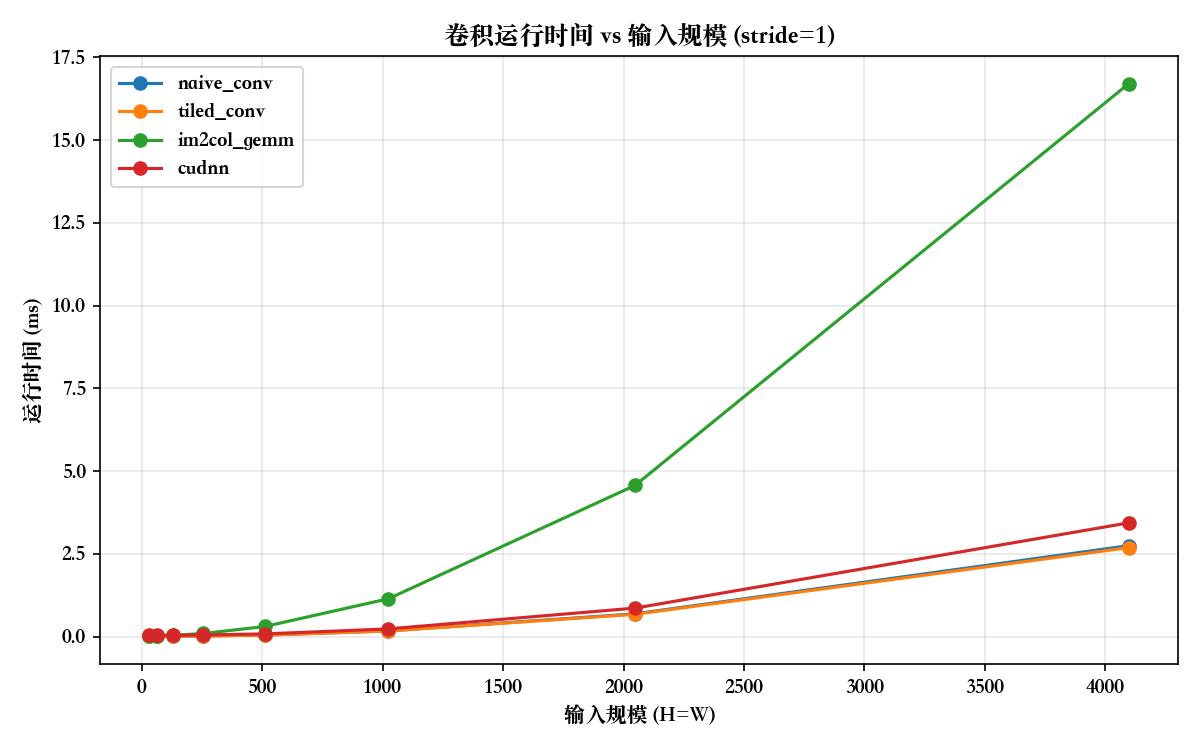
\includegraphics[width=0.85\textwidth]{runtime_vs_size.png}
  \caption{卷积运行时间随输入规模的变化（stride=1）}
  \label{fig:runtime}
\end{figure}

三种kernel在大规模下的性能排序为：tiled\_conv > naive\_conv > cuDNN > im2col\_gemm。
naive\_conv和tiled\_conv几乎重合，tiled仅领先2--3\%。im2col\_gemm在H$\ge$512后
明显掉队，cuDNN在所有规模下都慢于手写kernel。

\subsection{不同stride对性能的影响}

\begin{figure}[H]
  \centering
  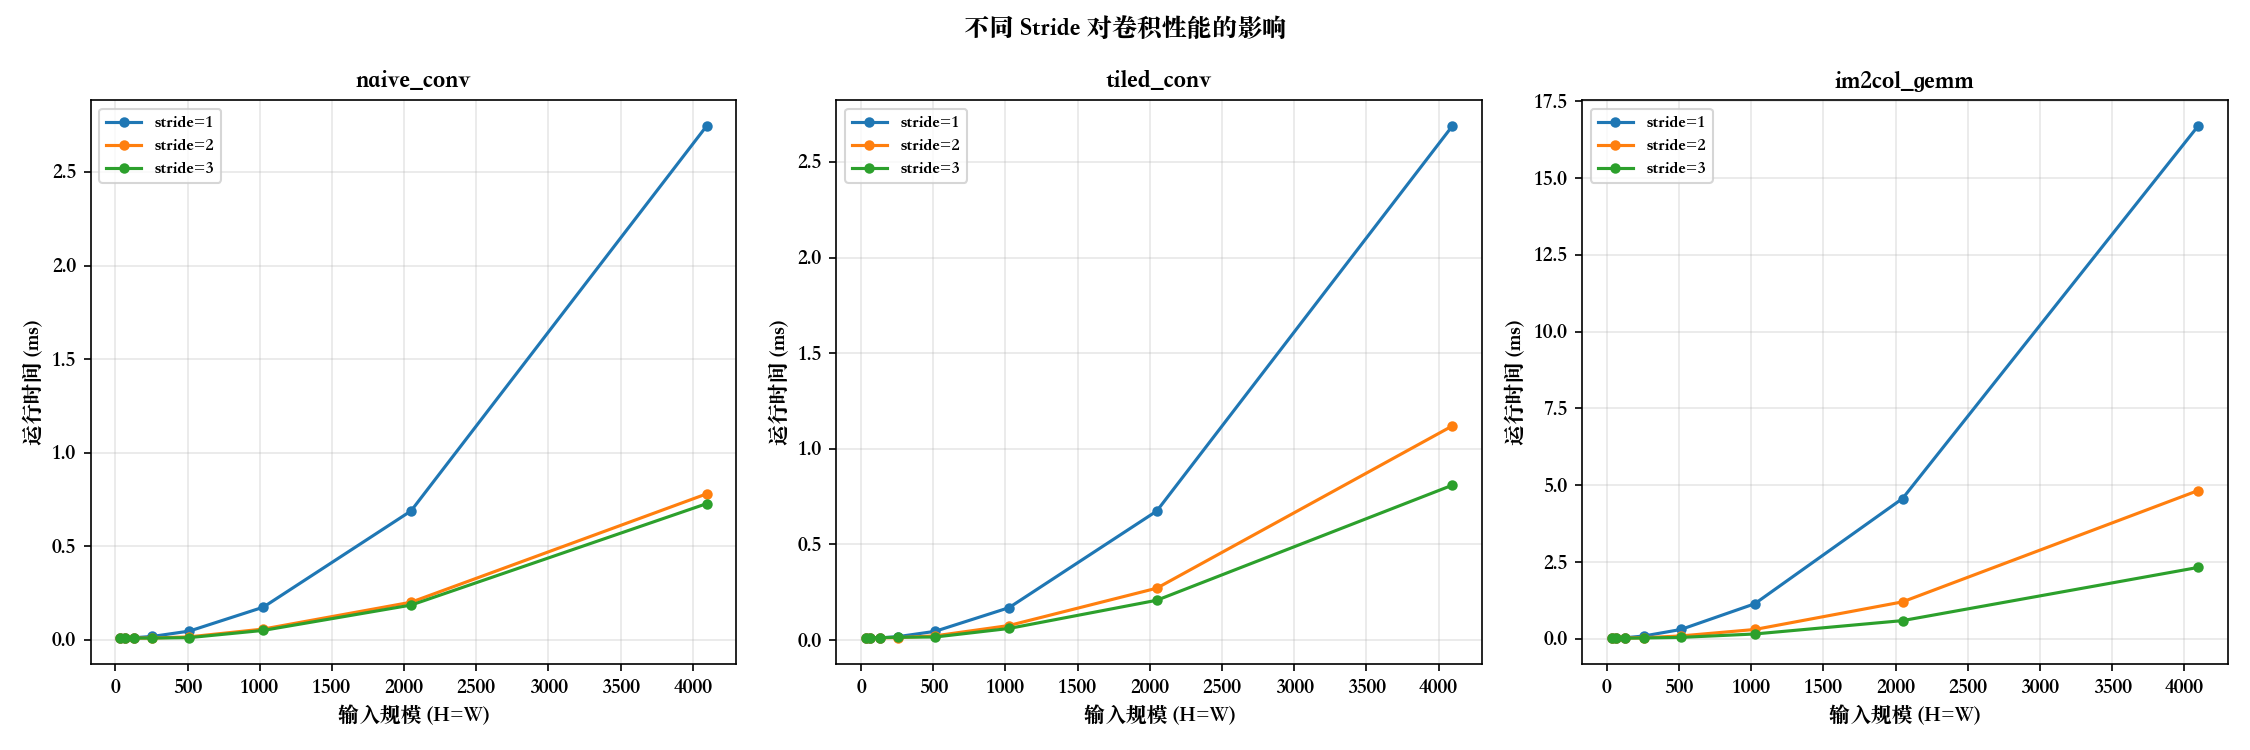
\includegraphics[width=0.95\textwidth]{stride_impact.png}
  \caption{不同stride下各kernel的运行时间}
  \label{fig:stride}
\end{figure}

stride增大主要降低输出尺寸，从而减少总计算量。H=4096时stride=3的naive\_conv仅需0.728ms
（stride=1时为2.75ms），减少了73\%。在stride=3且输入规模较小时，tiled\_conv反而
慢于naive\_conv（H=4096: 0.810ms vs 0.728ms），因为tile内有效线程占比降低，
halo加载的浪费比例增大。

\subsection{im2col时间分解}

\begin{table}[H]
  \centering
  \caption{im2col\_gemm时间分解（stride=1）}
  \label{tab:breakdown}
  \begin{tabular}{lcrr}
    \toprule
    H=W & 总时间(ms) & im2col(ms) 占比 & GEMM(ms) 占比 \\
    \midrule
    32   & 0.022  & 0.015 (69.1\%) & 0.006 (27.6\%) \\
    128  & 0.039  & 0.020 (52.6\%) & 0.018 (47.3\%) \\
    512  & 0.307  & 0.060 (19.7\%) & 0.246 (80.2\%) \\
    1024 & 1.144  & 0.174 (15.2\%) & 0.971 (84.9\%) \\
    4096 & 16.697 & 2.604 (15.6\%) & 13.426 (80.4\%) \\
    \bottomrule
  \end{tabular}
\end{table}

\begin{figure}[H]
  \centering
  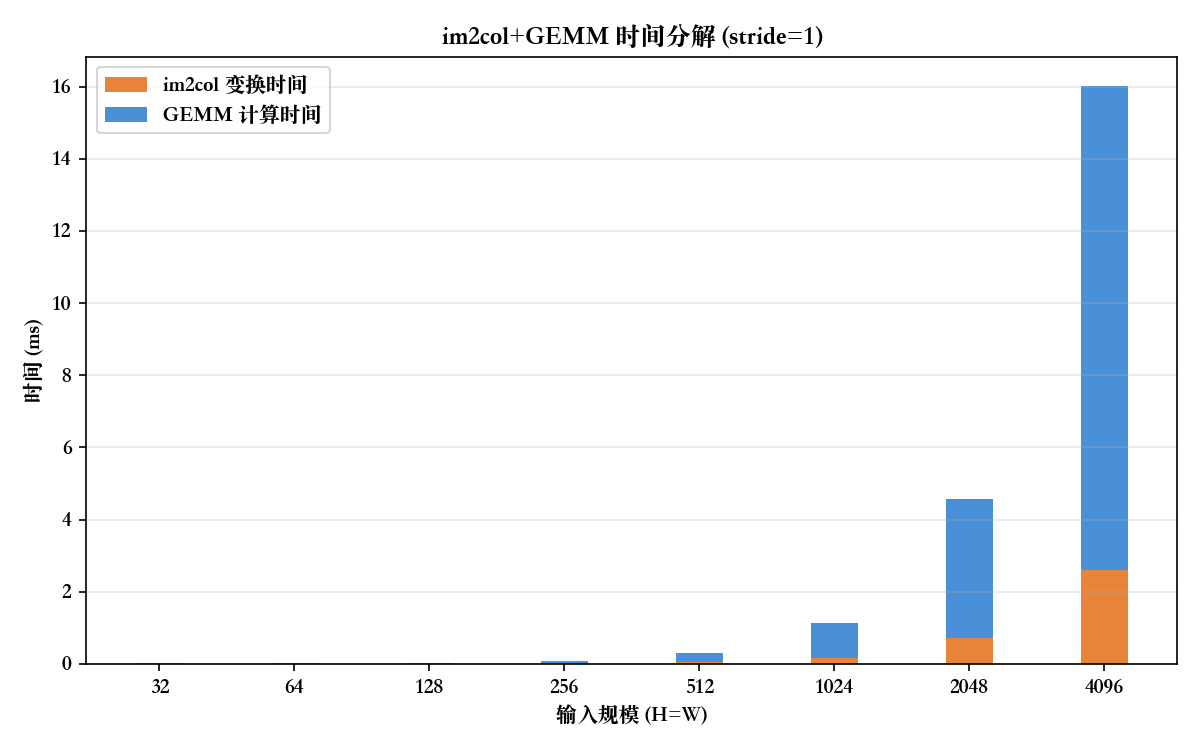
\includegraphics[width=0.80\textwidth]{time_breakdown.png}
  \caption{im2col+GEMM时间分解（stride=1）}
  \label{fig:breakdown}
\end{figure}

GEMM的时间占比从28\%（H=32）上升到80\%以上（H$\ge$512）。im2col变换的时间复杂度为
$O(C_{in} \cdot KH \cdot KW \cdot H_{out}W_{out})$，GEMM为
$O(C_{out} \cdot K \cdot H_{out}W_{out})$（$K=27$）。两者都是 $O(H_{out}W_{out})$，
但GEMM的常数因子更大且计算密集度更高，随着N增长更快地占据主导。
im2col变换本身高度并行——每个输出位置的展开完全独立，无依赖和同步。

\subsection{显存占用对比}

\begin{figure}[H]
  \centering
  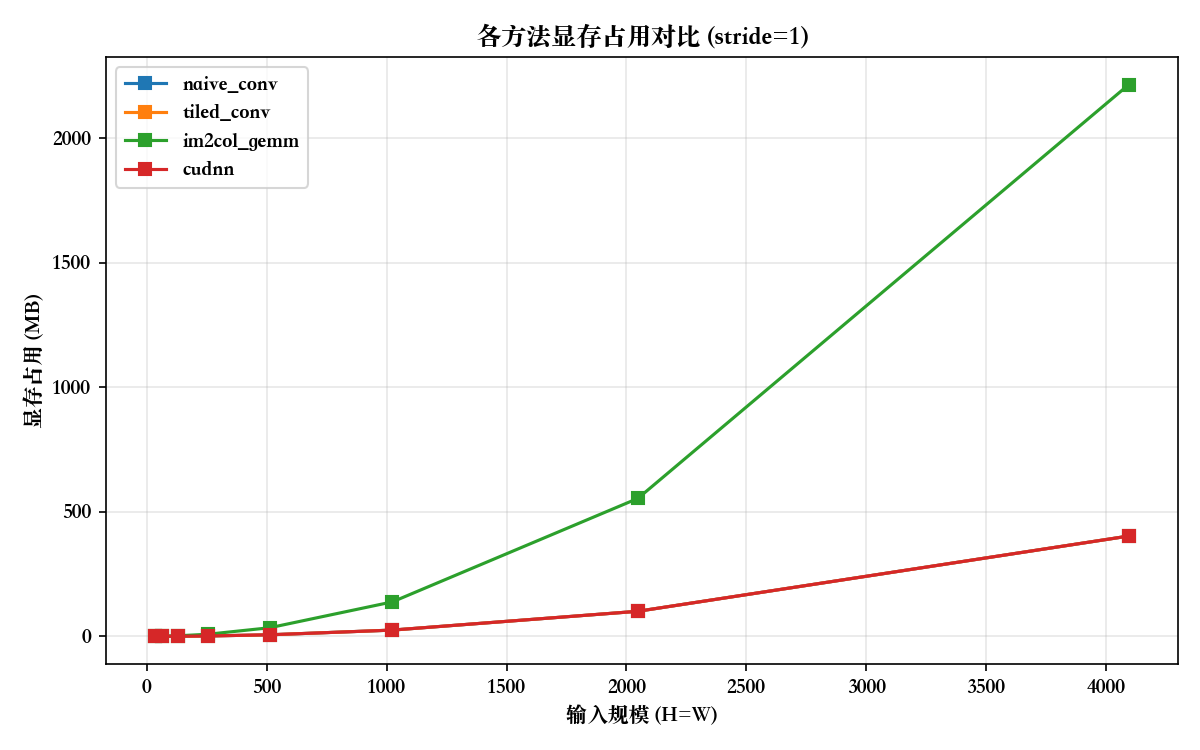
\includegraphics[width=0.85\textwidth]{memory_usage.png}
  \caption{各方法显存占用（stride=1）}
  \label{fig:memory}
\end{figure}

im2col\_gemm在H=4096时总显存约2.2 GB（含im2col矩阵1.81 GB），是其他方法的5.5倍。
naive、tiled和cuDNN仅需存储输入+权重+输出（约403 MB）。tiled\_conv的9KB共享内存
在SM上分配，不计入全局显存统计。

\subsection{加速比分析}

\begin{figure}[H]
  \centering
  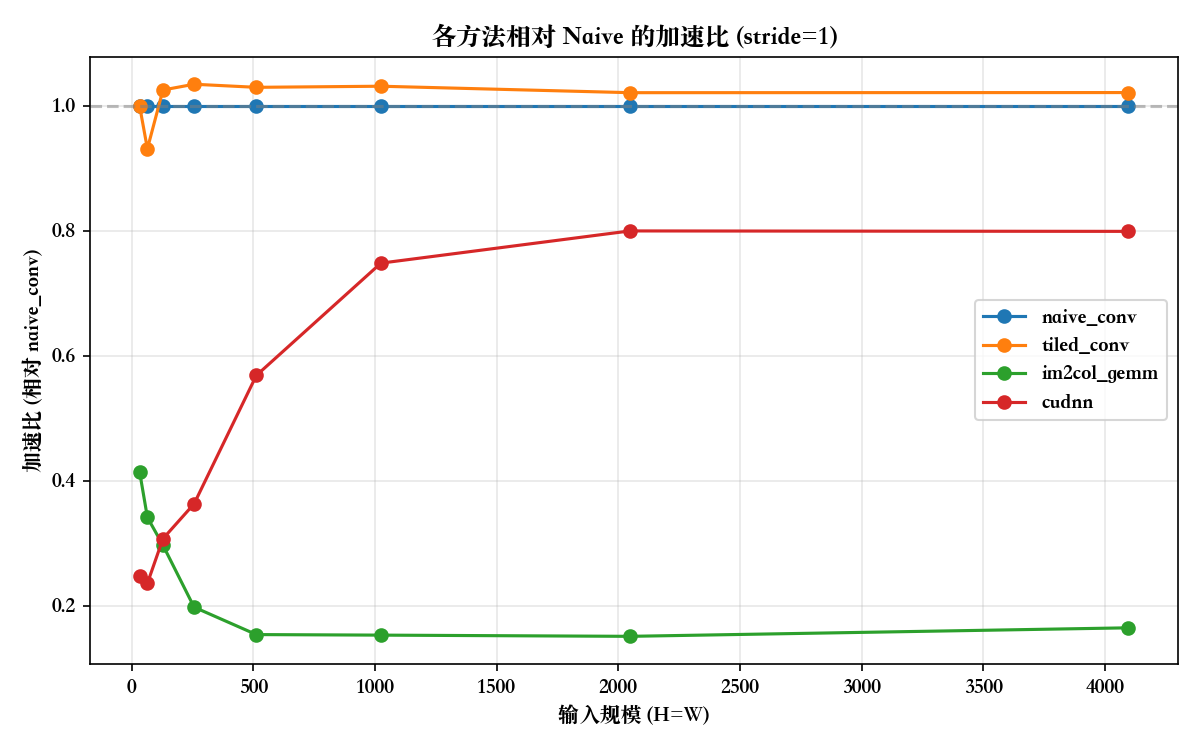
\includegraphics[width=0.85\textwidth]{speedup.png}
  \caption{各方法相对naive\_conv最佳配置的加速比（stride=1）}
  \label{fig:speedup}
\end{figure}

加速比呈现清晰的层次：
\begin{itemize}
  \item tiled\_conv在所有规模下 $\ge 1.0\times$，但最高仅1.03×；
  \item cuDNN从0.25×（H=32，启动开销占主导）随规模增大逐渐上升到0.80×（H=4096）；
  \item im2col\_gemm从0.41×（H=32）下降到约0.16×（H=4096），持续恶化。
\end{itemize}

\subsection{Block大小对Naive卷积的影响}

\begin{figure}[H]
  \centering
  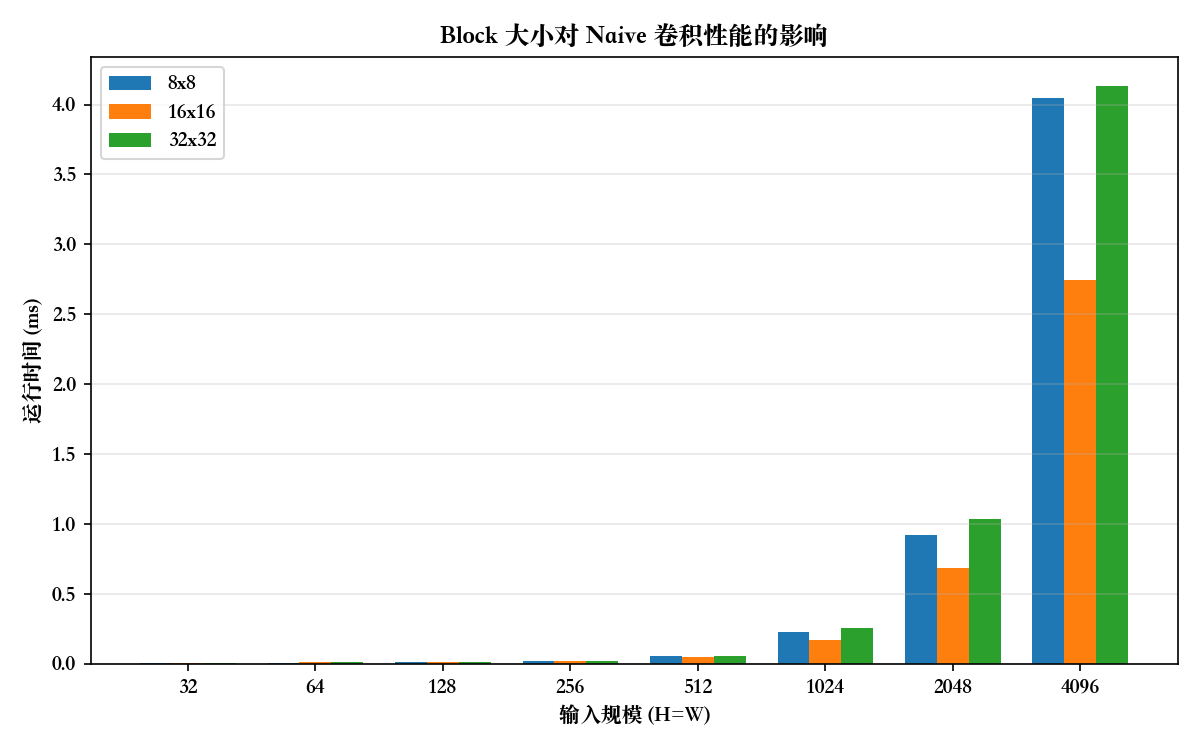
\includegraphics[width=0.85\textwidth]{block_size_impact.png}
  \caption{Block大小对Naive卷积的影响（stride=1）}
  \label{fig:blocksize}
\end{figure}

\begin{table}[H]
  \centering
  \caption{不同Block大小的Naive kernel性能（stride=1, ms）}
  \label{tab:blocksize_data}
  \begin{tabular}{lcccr}
    \toprule
    H=W & 8×8 & 16×16 & 32×32 & 16×16/最差比 \\
    \midrule
    256  & 0.0218 & \textbf{0.0187} & 0.0215 & 1.17× \\
    1024 & 0.2294 & \textbf{0.1747} & 0.2553 & 1.46× \\
    4096 & 4.0472 & \textbf{2.7460} & 4.1359 & 1.51× \\
    \bottomrule
  \end{tabular}
\end{table}

与Lab9和Lab10结论一致：16×16在所有规模下最优。8×8每block仅2个warp导致延迟隐藏不足；
32×32虽有32个warp的最强延迟隐藏能力，但每SM仅1个block使block级并行度为零。

\subsection{运行时间热力图}

\begin{figure}[H]
  \centering
  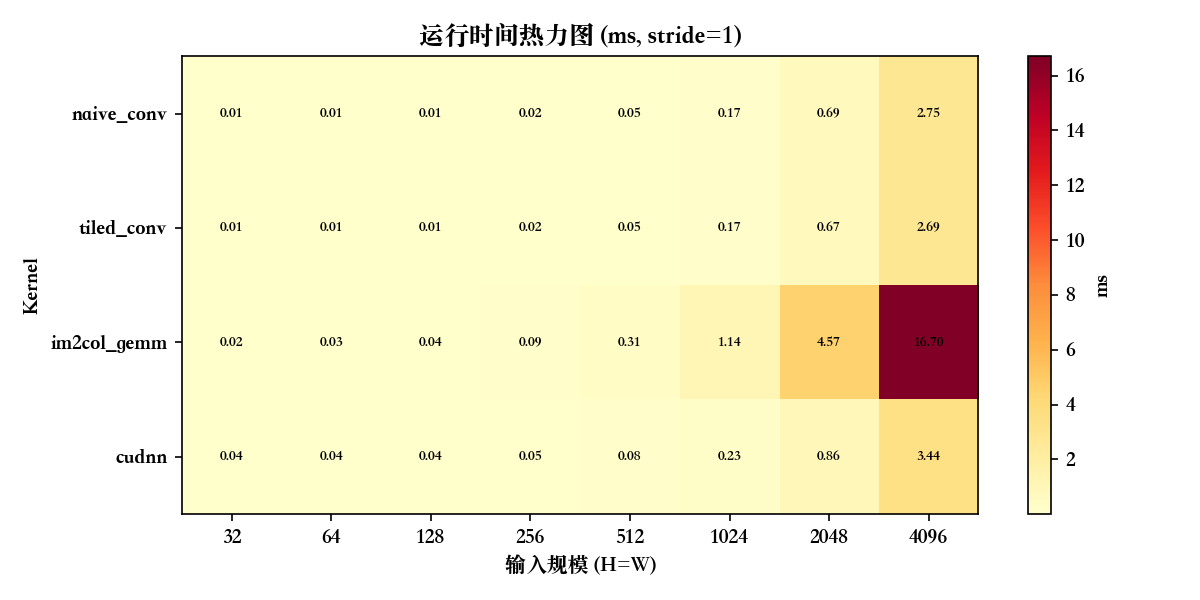
\includegraphics[width=0.85\textwidth]{heatmap.png}
  \caption{运行时间热力图（规模 × Kernel, stride=1, ms）}
  \label{fig:heatmap}
\end{figure}

\section{讨论}

\subsection{tiled\_conv为什么几乎没加速？——3×3卷积的特异性}

tiled\_conv理论上通过共享内存分块复用输入数据，可减少约4×的全局内存访问
（相邻输出共享约93\%的输入元素）。实测仅获得2--3\%的提升，原因与3×3小kernel相关：

\begin{itemize}
  \item 每个输出元素的27次乘加仅54 FLOPs。RTX 3090的理论FP32峰值35.6 TFLOPS
        和936 GB/s带宽下，roofline拐点在约38 FLOP/byte。3×3卷积仅约0.2 FLOP/byte，
        远在内存带宽bound区，计算单元大量空闲；
  \item 在内存带宽bound的情况下，减少全局内存读取的收益被共享内存访问
        和\_\_syncthreads()额外的开销几乎完全对冲；
  \item 如果卷积核增大到5×5或7×7，tiling的收益会更加明显——更大kernel意味着
        更少的数据复用率，tiling节省的相对访存量更大。
\end{itemize}

\subsection{cuDNN为什么比手写kernel慢？}

这是本次实验最反直觉的结果。实测cuDNN比tiled\_conv慢约28\%（H=4096时），
差距随规模减小而更大（表\ref{tab:cudnn_vs_tiled}）。

\begin{table}[H]
  \centering
  \caption{cuDNN与tiled\_conv性能差距（stride=1）}
  \label{tab:cudnn_vs_tiled}
  \begin{tabular}{lccr}
    \toprule
    H=W & tiled\_conv (ms) & cuDNN (ms) & cuDNN慢(\%) \\
    \midrule
    32   & 0.0092 & 0.0372 & +303.9\% \\
    128  & 0.0113 & 0.0376 & +233.6\% \\
    512  & 0.0457 & 0.0828 & +81.2\% \\
    1024 & 0.1694 & 0.2335 & +37.8\% \\
    2048 & 0.6748 & 0.8615 & +27.7\% \\
    4096 & 2.6883 & 3.4359 & +27.8\% \\
    \bottomrule
  \end{tabular}
\end{table}

原因分析：

\begin{enumerate}
  \item \textbf{sm\_37编译目标}：nvcc 10.0将kernel编译为sm\_37（Kepler, 2012年）的PTX，
        GPU驱动在运行时JIT编译为Ampere（2020年）原生指令。cuDNN 8.9.7的内部kernel
        同样受限于此——对Ampere的优化（tensor core、async copy等）在跨代JIT中无法利用；
  \item \textbf{固定IMPLICIT\_GEMM算法}：为了避免\texttt{cudnnFindConvolutionForwardAlgorithm}
        在平台上的hang问题，固定使用单一算法。其他算法（如WINOGRAD）可能更适合3×3卷积；
  \item \textbf{CUDA Runtime版本分裂}：nvcc 10.0静态链接了Runtime 10.0，而cuDNN 8.9.7
        依赖libcudart.so.12。两个版本的Runtime共存可能引入内部状态差异。
\end{enumerate}

差距随规模增大而缩小（从304\%到28\%），说明cuDNN的框架开销（描述符创建、workspace分配等）
在小规模时占主导。这一现象提醒我们：在受限平台上，库函数未必是最优选择，
直接实现反而可能因为简洁而获得更好的性能。

\subsection{im2col方案的实际适用场景}

im2col\_gemm在所有测试中都是最慢的方案，但这不意味着im2col本身不好。
它在以下场景会更有竞争力：

\begin{itemize}
  \item 使用高度优化的GEMM库（如cuBLAS cublasSgemm）替换手写tiled GEMM；
  \item 卷积核尺寸更大（5×5或7×7），$K$增大后GEMM的计算密度更高；
  \item batch size > 1，im2col可批量处理多张输入，摊销变换开销。
\end{itemize}

在本次实验的单样本、3×3小kernel场景下，im2col变换开销和手写GEMM的不足共同导致了
其性能劣势，这是预期内的结果。

\section{验证与测试}

所有kernel均通过CPU参考验证（对于H=W$\le$256的输入逐元素对比）和checksum验证
（同一配置下所有kernel的checksum一致，允许$<10^{-4}$的浮点误差）。
benchmark中所有配置均输出\texttt{correct=true}，四种kernel数值上完全等价。

图~\ref{fig:terminal} 展示了在智算习堂平台上的实验过程。

\begin{figure}[H]
  \centering
  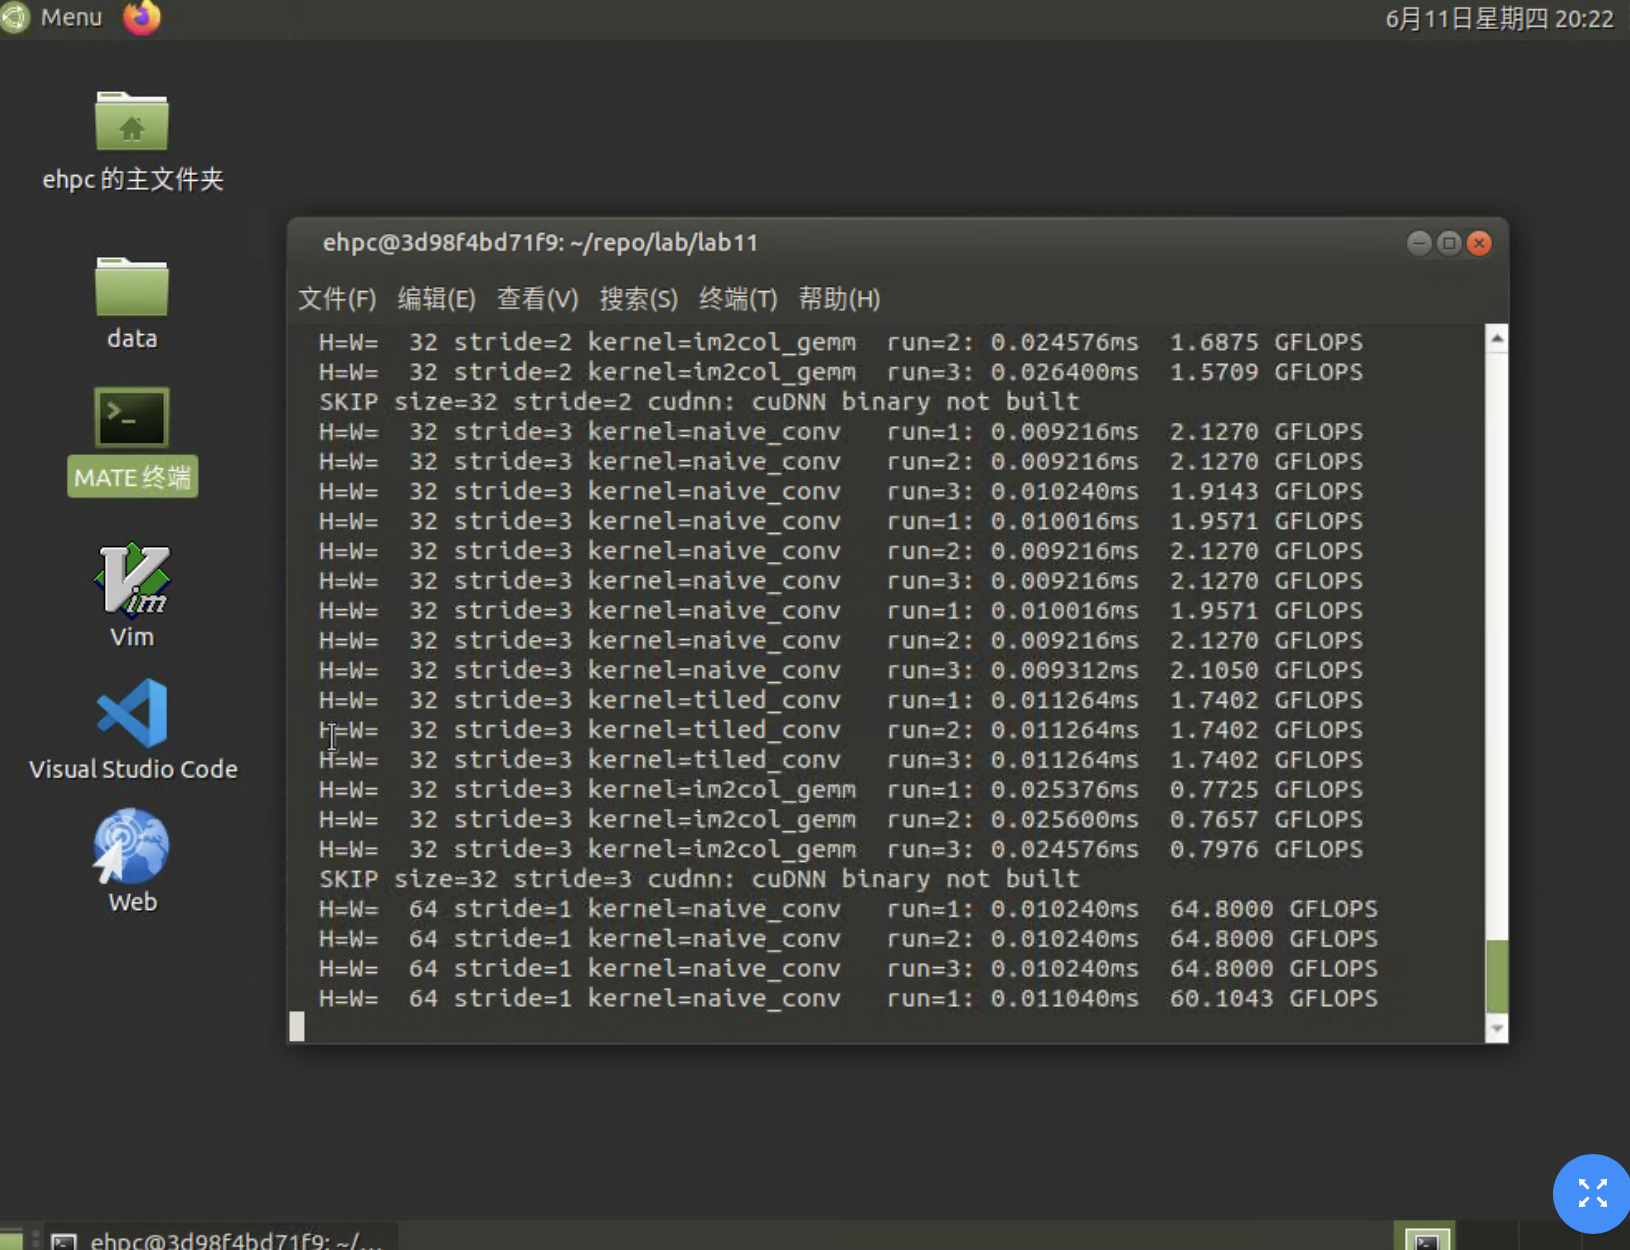
\includegraphics[width=\textwidth]{terminal_screenshot.png}
  \caption{智算习堂平台实验终端截图（编译、单次测试、benchmark运行）}
  \label{fig:terminal}
\end{figure}

\section{结论}

本次实验使用CUDA实现了四种CNN卷积计算方法，在智算习堂RTX 3090上完成了
覆盖8种输入规模、3种stride的benchmark测试。主要结论：

\begin{enumerate}[leftmargin=2.2em]
  \item 在3×3小卷积核下，tiled\_conv仅比naive\_conv快2--3\%。小kernel使得计算/访存比
        极低（约0.2 FLOP/byte），操作处于内存带宽bound，共享内存tiling的访存收益
        被同步开销抵消。这一结果为理解"优化策略的有效性取决于问题特征"提供了具体例证。
  \item cuDNN在sm\_37编译目标下并未表现出性能优势，反而比tiled\_conv慢约28\%
        （H=4096时）。编译器与GPU代际不匹配是主要原因。这提醒我们使用GPU库函数前
        应确认CUDA Toolkit与硬件的版本对应关系。
  \item 16×16是最优block大小，与Lab9、Lab10的结论一致，验证了这一配置在
        RTX 3090 Ampere架构上的普适性。
  \item im2col\_gemm由于额外显存开销（5.5×）和手写GEMM的限制，在本次配置下竞争力不足，
        但其时间分解结果验证了im2col变换开销随规模增大而占比下降的理论预测。
  \item 实验成功通过pip安装新版cuDNN 8.9.7和CUDA Runtime 12.x，在CUDA Toolkit 10.0
        的受限平台上实现了RTX 3090的cuDNN支持，为类似受限环境提供了可参考的技术路线。
\end{enumerate}

\end{document}
